\DocumentMetadata{
  pdfversion=2.0,
  lang=es-MX,
  pdfstandard=ua-2
}

\documentclass{sener2025}

% --- Metadatos PDF/UA (Accesibilidad Universal) ---
\hypersetup{
  pdftitle={Demo Latex y Fucnionalidades X},
  pdfauthor={SENER},
  pdfsubject={BNE 2025},
  pdfkeywords={Energías},
  pdfcreationdate={D:20251219161706}
}

% --- Metadatos del Documento ---
\title{Demo Latex y Fucnionalidades X}
\subtitle{BNE 2025}
\author{SENER}
\date{17 de diciembre de 2025}
\institucion{Secretaría de Energía (SENER)}
\unidad{Unidad de Planeación y Transición Energética}
\setDocumentoCorto{Demo2}
\palabrasclave{Energías}
\version{1}

\begin{document}

\portadafondo[img/portada.jpg]

\tableofcontents
\newpage

\listafiguras
\newpage

\listatablas
\newpage

\clearpage
\begin{center}
{\Large\patriafont\bfseries\color{gobmxGuinda}Presentación}\\[1cm]
\end{center}

La Seguridad Energética es un objetivo estratégico del Plan Nacional de Desarrollo 2025-2030, pero debe hacerse con una visión de sustentabilidad ambiental; para ello es fundamental consolidar la rectoría del Estado en el sector energético mediante el fortalecimiento de PEMEX y de la CFE. Esto permitirá eliminar la dependencia del exterior, asegurar precios accesibles para la población y avanzar hacia la autosuficiencia energética. En la matriz energética del país se impulsarán fuentes de energía renovables y se acelerará la transición energética con el objetivo de reducir las emisiones contaminantes, cumplir con las metas nacionales de energías limpias y honrar los compromisos internacionales en la lucha contra el cambio climático.

Además de garantizar un suministro energético seguro, eficiente y asequible para toda la población, la justicia energética debe convertirse en un pilar del desarrollo nacional. Esto implica ampliar la cobertura y el acceso a la energía, especialmente en comunidades marginadas, asegurando que todas las regiones del país cuenten con fuentes de energía limpias y sostenibles.

En México se ha tomado la decisión de trabajar con una visión de preservar la seguridad y autosuficiencia energética, encaminarse a una transición energética justa y sustentable, así como de brindar certeza jurídica a las actividades que se realizan en el sector. Por estas razones, se han hecho cambios al marco jurídico del sector energético partiendo de las modificaciones a la Constitución Política de los Estados Unidos Mexicanos y a diversos ordenamientos jurídicos que de ella emanan. En este sentido, la SENER tiene el mandato legal de ser el órgano rector de la política y planeación energética nacional, bajo criterios de soberanía y seguridad energética, autosuficiencia, restitución y aumento de reservas, diversificación de fuentes de combustibles, mejoramiento de la productividad, la reducción progresiva de impactos ambientales en la producción y consumo de energía, y la satisfacción de las necesidades energéticas básicas mediante cobertura universal a toda la población a precios accesibles.

\portadaseccion{1}{Introducción}{}

\section{Introducción}

El sector energético es un área estratégica para el funcionamiento de la economía y el bienestar de la sociedad mexicana, ya que proporciona energía para el desarrollo nacional a través de diversos sectores productivos (agropecuario, industrial, residencial, comercial, transporte, de servicios públicos, entre otros). También, suministra insumos para fines no energéticos en la industria petroquímica, como es la producción de fertilizantes, medicamentos y plásticos ampliamente utilizados en un sin número de artículos de uso cotidiano.
Con el propósito de comprender y analizar la dinámica energética del país, así como de generar la base para la planeación vinculante, la Secretaría de Energía (SENER) elabora anualmente el Balance Nacional de Energía (BNE). Actualmente, este instrumento se desarrolla en el marco de la Reforma Energética de 2025, lo que le confiere un papel fundamental en la definición de políticas y estrategias para el Sector Energético Mexicano (SEM).
En este documento no solo se analiza el desempeño del SEM en el año 2024, sino que se detalla el periodo 2010 - 2024 a fin de comprender su comportamiento histórico. Por lo tanto, este documento describe las fuentes de energía, su extracción y producción, transformación a productos energéticos secundarios y el consumo final de estos. A partir de ello, el BNE busca evaluar la dinámica de cada elemento en la cadena de valor del sector energético y poner a disposición del público información valiosa para el desarrollo del mismo.
Además, esta información es esencial para desarrollar los instrumentos de planeación del sector energético, evaluar su desempeño, así como para el diseño de políticas públicas y la toma de decisiones estratégicas alineados al Plan Nacional de Desarrollo (PND) 2025-2030 y al Programa Sectorial de Energía (PROSENER) 2025-2030.
El BNE se basa únicamente en un análisis energético, por lo que excluye aspectos económicos como el Producto Interno Bruto (PIB), los precios y las tarifas de la energía o la inflación. Esto se debe a que el documento ofrece un panorama general sobre el sector energético a partir de las bases energéticas objetivas con las que cuenta el país, con lo que se ofrece, no solo una visión del presente, sino una proyección del futuro energético de México.\footnote{esta es una nota}

Figura:
% Referencia a figura: FIG-1-1

Cita:
\cite{inventarioGEI2024}


\subsection{Fundamento jurídico del Balance Nacional de Energía [[nota:Prueba]]}

Ejemplo de \footnote{Ejemplo}

Figura:
% Referencia a figura: FIG-1.1-1

Tabla
% Referencia a tabla: TBL-1.1-1
\begin{figure}[H]
  {\centering
  % Texto alternativo para accesibilidad
  \pdftooltip{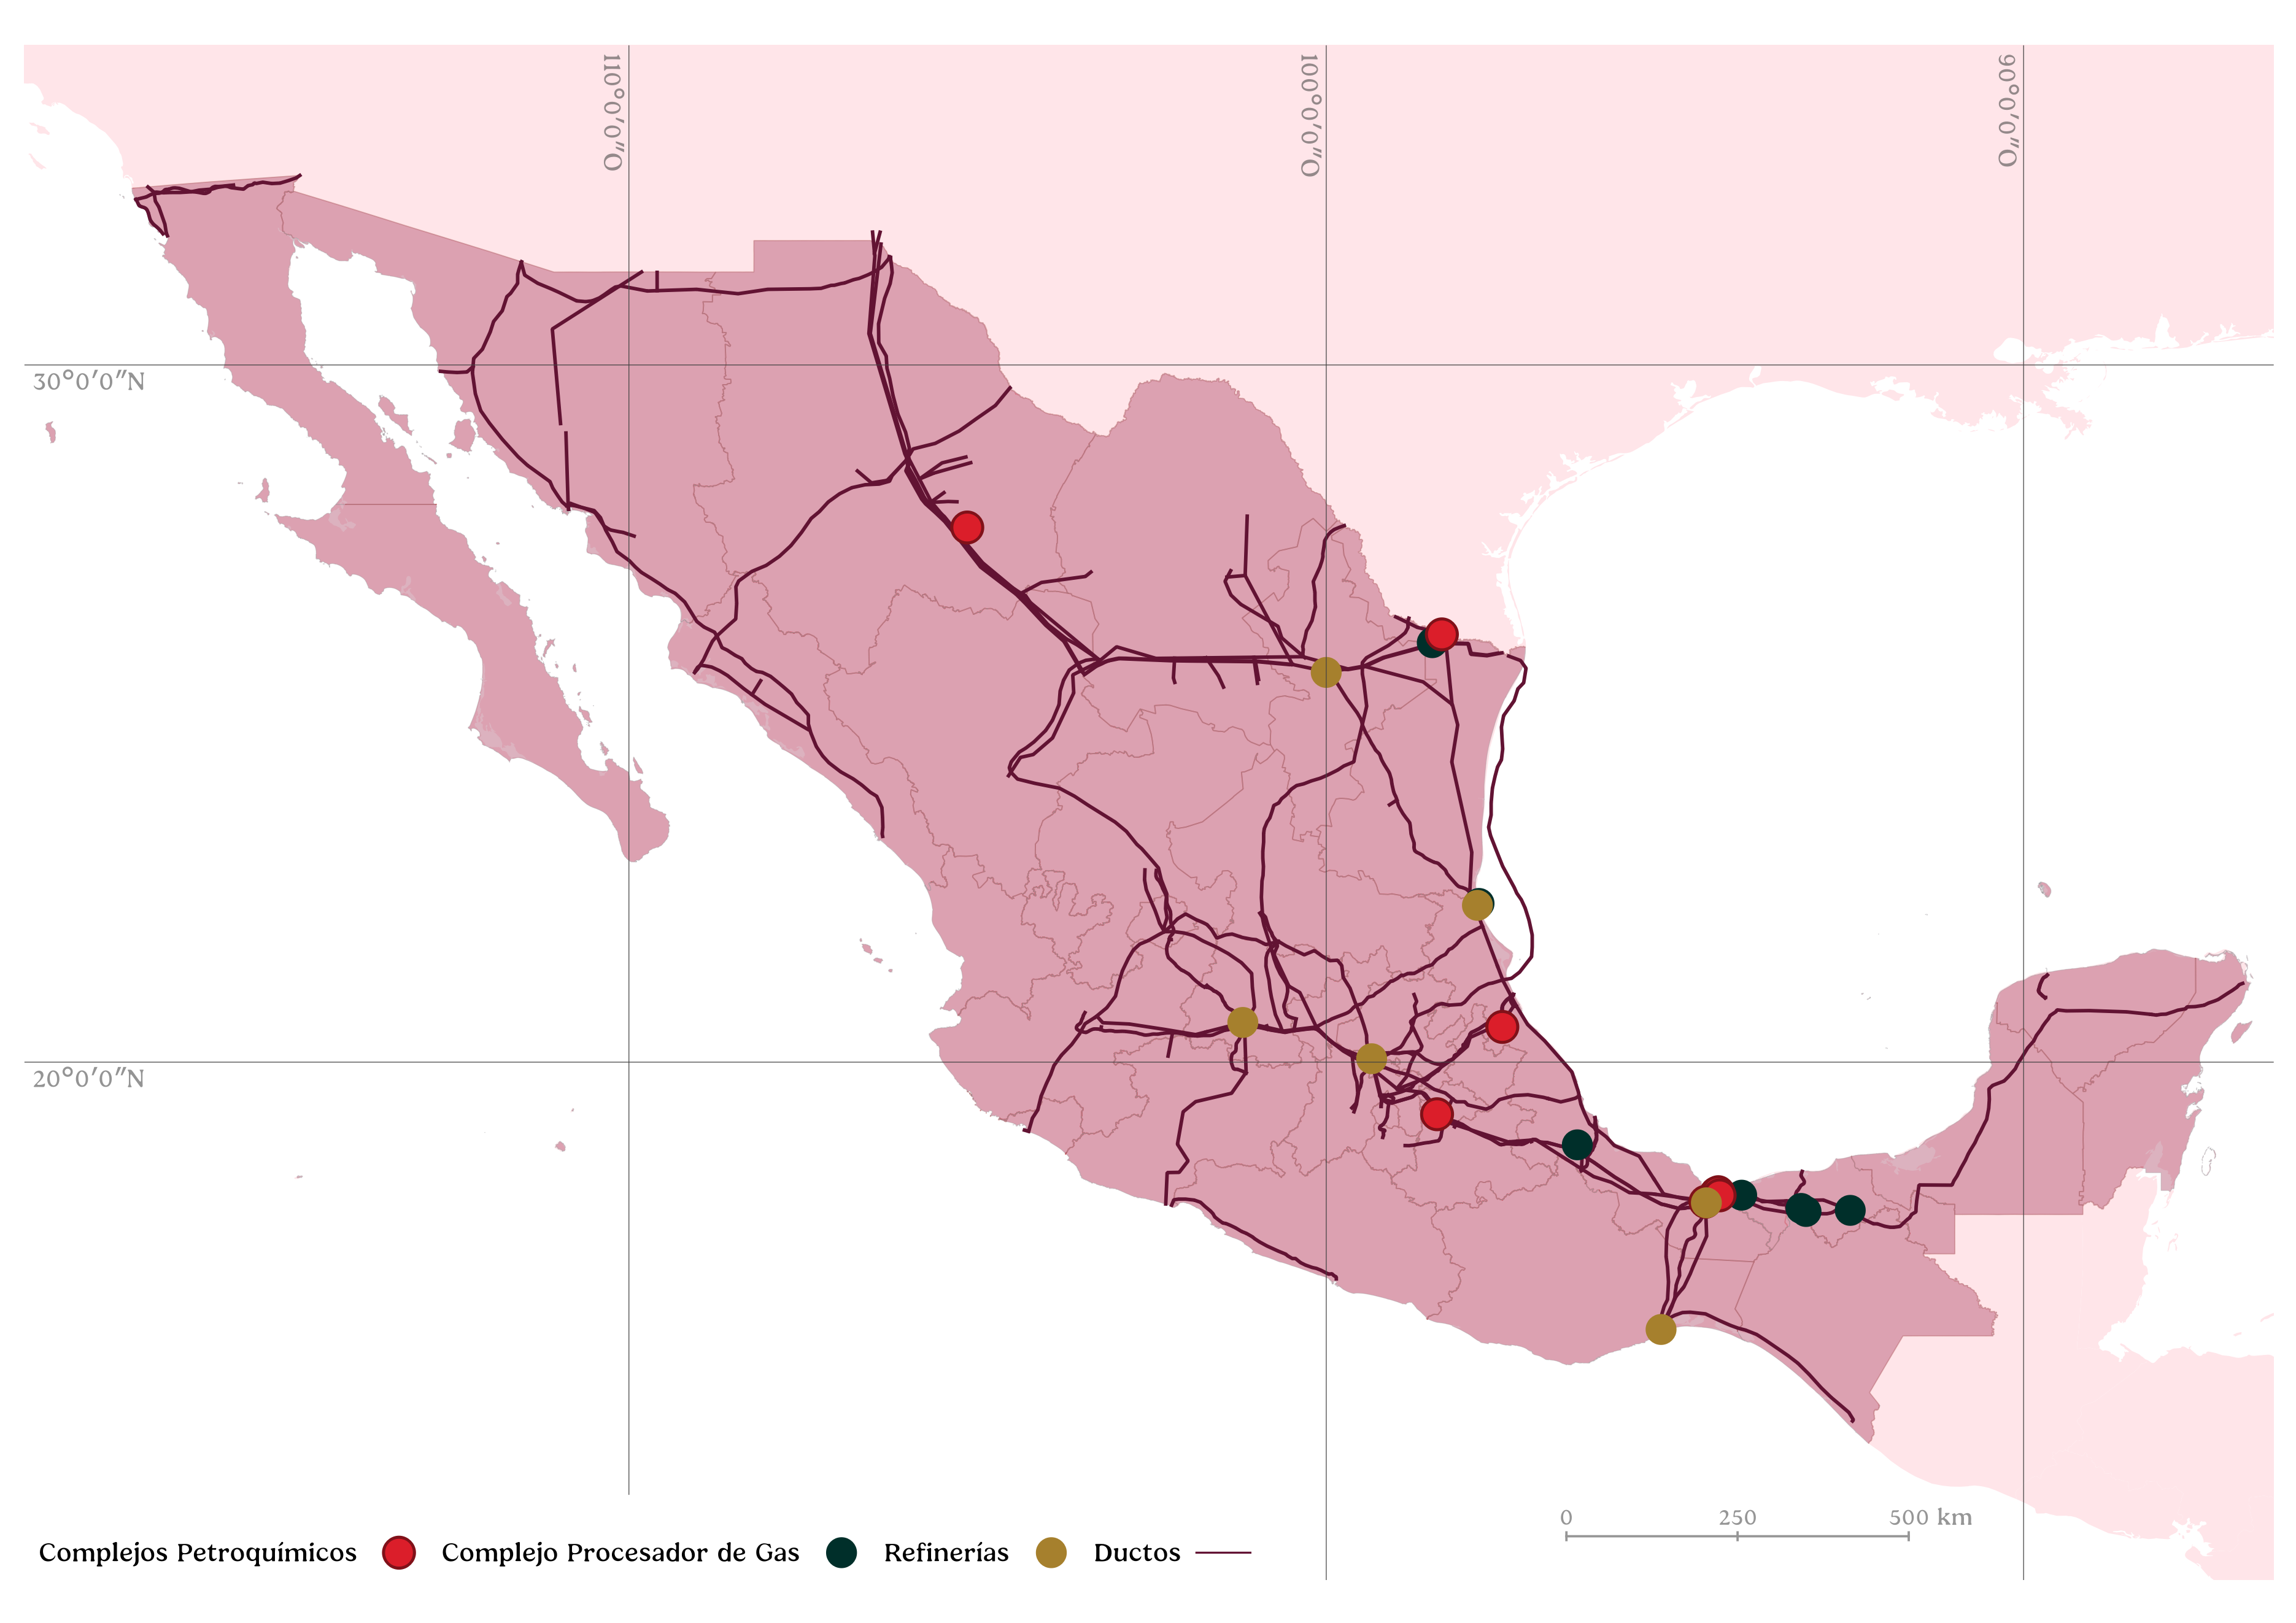
\includegraphics[width=0.8\textwidth]{img/figura_2_1.png}}{Figura 1.1 Principal infraestructura del sector hidrocarburos, 2024}
  \par}
  \raggedright
  \caption{Figura 1.1 Principal infraestructura del sector hidrocarburos, 2024 }
  \label{fig:figura_1_1_principal_infraestr}
\end{figure}
\vspace{-4pt}
\fuente{Elaboración SENER.[[nota:Nota Fuente]]}

\begin{tabladoradoCorto}
  \caption{Tabla 1.1 Reservas de Hidrocarburos de la Nación, 2024 }
  \label{tab:tabla_1_1_reservas_de_hidrocar}
  \begin{tabularx}{\textwidth}{Vvvv}
    \toprule
    \rowcolor{gobmxDorado} \encabezadodorado{CATEGORIA [[nota:Prueba]]} & \encabezadodorado{ACEITE 
(MMb)} & \encabezadodorado{GAS 
(MMMpc)} & \encabezadodorado{} \\
    \midrule
    Total 1p & 5,978 & 12,297 & 8,383 \\
    Total 2P & 11,078 [[nota:Prueba]] &  & 15,530 \\
    Total 3P & 16,383 & 34,858 & 23,146 \\
    \bottomrule
  \end{tabularx}
\end{tabladoradoCorto}
\vspace{-4pt}
\fuente{Elaboración de SENER con información del Sistema de Información de Hidrocarburos de la SENER, Reservas al 01 de enero de 2024}



\section*{Glosario}
\phantomsection
\addcontentsline{toc}{section}{Glosario}

\entradaGlosario{Bagazo de caña}{Energético primario compuesto de material fibroso resultante después de la extracción de jugo en la última molienda, así como otros materiales orgánicos provenientes de la cosecha de la propia caña.}
\entradaGlosario{Biocombustible}{Son los combustibles en estado gaseoso, líquido o sólido que se obtienen a partir del aprovechamiento energético directo de la biomasa o mediante su transformación física, química o biológica.
No se consideran biocombustibles las mezclas con derivados del petróleo (petrolíferos), incluso si contienen una fracción de origen biológico.}
\entradaGlosario{Biogás}{Es un energético primario en estado gaseoso, producido a partir de la descomposición anaeróbica de biomasa y/o de la fracción biodegradable de los residuos. Su composición permite que, tras un proceso de purificación, pueda usarse como biocombustible o como sustituto del gas natural en aplicaciones energéticas principalmente en generación de energía eléctrica y calefacción.}
\entradaGlosario{Carboeléctrica}{Instalaciones que queman carbón para producir vapor con el fin de generar energía eléctrica.}
\entradaGlosario{Carbón mineral}{Es un energético primario en estado sólido, de color negro o marrón, que contiene esencialmente carbono, pequeñas cantidades de hidrógeno, oxígeno, nitrógeno, azufre y otros elementos, el cual proviene de la degradación de organismos vegetales durante un largo periodo de tiempo.}
\entradaGlosario{Central Eléctrica}{Instalación destinada a la generación de energía eléctrica a través de la conversión de energía mecánica, obtenida a partir de diversas fuentes de energía primaria, tales como combustibles fósiles, energía hidráulica, nuclear, eólica, solar fotovoltaica, entre otras. Estas instalaciones integran sistemas de conversión energética que incluyen turbinas, generadores eléctricos y equipos auxiliares para transformar y optimizar la producción eléctrica conforme a los requerimientos de la red de suministro.}
\entradaGlosario{Centros de Transformación}{Instalaciones industriales de transformación de la energía primaria en productos energéticos secundarios con características que permiten su uso o consumo final.}
\entradaGlosario{Ciclo Combinado}{Tecnología de generación eléctrica que integra dos ciclos termodinámicos complementarios para maximizar la eficiencia energética. Una turbina de gas convierte la energía química del combustible en energía mecánica a alta temperatura y presión, generando electricidad de manera directa. Los gases de escape calientes resultantes de esta turbina no se desperdician, sino que se canalizan hacia una caldera de recuperación de calor, donde se produce vapor de alta presión. Este vapor alimenta una turbina de vapor de condensación, que convierte la energía térmica residual en energía mecánica adicional, incrementando la producción eléctrica total sin aumentar significativamente el consumo de combustible.}
\entradaGlosario{Cogeneración}{Generación de energía eléctrica producida de manera conjunta con vapor u otro tipo de energía térmica secundaria útil o ambos; producción directa o indirecta de energía eléctrica mediante la energía térmica no aprovechada en los procesos, o generación directa o indirecta de energía eléctrica cuando se utilicen combustibles producidos en los procesos industriales.}
\entradaGlosario{Cogeneración Eficiente}{Es la generación de energía eléctrica usando en conjunto una energía térmica secundaria.}
\entradaGlosario{Combustión interna}{Principio de fundamento empleado en centrales eléctricas que utilizan motores de combustión interna, generalmente basados en la tecnología de motores diesel, y alimentados por combustibles líquidos como combustóleo o diesel. En estos sistemas, la energía química del combustible se convierte en energía térmica mediante un proceso de combustión controlada dentro de los cilindros del motor. La rápida expansión de los gases de combustión generados produce un movimiento lineal o rotativo en los pistones, transformando la energía térmica en energía mecánica. Esta energía mecánica es transmitida a un generador eléctrico que, a través de un sistema electromagnético, convierte el movimiento rotatorio en energía eléctrica.}
\entradaGlosario{Combustóleo}{Energético secundario compuesto por una mezcla compleja de hidrocarburos pesados con una concentración de fracciones residuales de alto peso molecular, generado durante las etapas finales de la refinación del petróleo. Debido a su alta viscosidad y contenido de compuestos sulfatados, es comúnmente empleado en calderas industriales y procesos de generación térmica que toleran combustibles de menor calidad.}
\entradaGlosario{Consumo final}{Es la energía y materia prima que funge como combustible destinado a los diferentes sectores de  la economía para su consumo, de este mismo se deriva el consumo final no energético y el consumo final energético.}
\entradaGlosario{Consumo final energético}{Es el aprovechamiento de la energía primaria y secundaria para atender las necesidades energéticas de los sectores de consumo; Agropecuario, industrial, comercial, residencial público y transporte.}
\entradaGlosario{Consumo final no energético}{Es el uso de energéticos primarios y secundarios como insumos en procesos industriales que no tienen como fin la generación de energía, sino la transformación de materias primas para la elaboración de productos no energéticos. Este tipo de consumo es común en sectores como la industria petroquímica, donde se utilizan hidrocarburos para fabricar plásticos, fertilizantes, solventes u otros productos químicos.}
\entradaGlosario{Consumo propio del sector energético}{Es el consumo de energía primaria y secundaria utilizado internamente por las propias instalaciones del sector energético, incluyendo plantas de extracción, procesamiento, transformación, transporte y distribución. Este consumo no se destina a los usuarios finales, sino que es necesario para operar los sistemas que hacen posible la generación, conversión y entrega de energía.}
\entradaGlosario{Coque de carbón}{Es un energético secundario, proveniente de la coquización del carbón bituminoso en plantas de coque. Se produce al someter el carbón siderúrgico a un proceso de calentamiento controlado en ausencia de oxígeno. Durante este tratamiento térmico, se eliminan los componentes volátiles del carbón, dando lugar a un material rico en carbono, con alta resistencia mecánica y capacidad calorífica.}
\entradaGlosario{Coque de petróleo}{Es un energético secundario sólido producido en la etapa de coquización dentro del proceso de refinación del petróleo crudo. Se genera un residuo carbonoso con alto contenido de carbono y bajo en hidrógeno, resultado de la descomposición térmica controlada de fracciones pesadas residuales a temperaturas elevadas.}
\entradaGlosario{Coquizadoras y hornos}{Plantas de procesos donde se obtiene coque de petróleo y carbón como resultado de la combustión del carbón mineral y de otros materiales carbonosos.}
\entradaGlosario{Diesel}{Es un energético secundario en estado líquido obtenido principalmente de la destilación del petróleo a una temperatura entre los 200°C y 380°C, este se llega a clasificar dependiendo a su uso, si es para vehículos, maquinaria agrícola o uso específicamente para calderas o que generan calor debido a su alto contenido de parafinas.}
\entradaGlosario{Diferencia estadística}{En el balance energético, la diferencia estadística representa la discrepancia numérica entre la oferta total energética y su consumo final. Esta diferencia se calcula restando el consumo final de la oferta total.}
\entradaGlosario{Energía eléctrica}{Es la energía producida por el desplazamiento de cargas eléctricas principalmente electrones, a través de un conductor. Este flujo de cargas se produce como consecuencia de una diferencia de potencial eléctrico entre dos puntos, la cual establece un campo eléctrico que induce el movimiento ordenado de dichas cargas. Este desplazamiento permite la realización de trabajo eléctrico.}
\entradaGlosario{Energía eólica}{Es la energía primaria obtenida a partir de la conversión de la energía cinética del viento, producida por el desplazamiento de las corrientes de aire ocasionadas por el calentamiento no uniforme de la superficie terrestre.}
\entradaGlosario{Energía geotérmica}{Energía primaria extraída del calor interno de la tierra,  concentrado en sistemas o yacimientos geotérmicos subterráneos. Este calor se manifiesta en la superficie a través de manantiales, suelos calientes, volcanes de lodo, fumarolas, géiseres y zonas de alteración hidrotermal.}
\entradaGlosario{Energía hidráulica}{Es la energía primaria obtenida a partir de la transformación de la energía potencial y cinética del agua en movimiento, proveniente de la circulación natural de masas líquidas en ríos o arroyos, que fluyen desde zonas elevadas o montañosas hacia áreas de menor latitud, como llanuras o costas. Esta energía es aprovechada para generar electricidad mediante sistemas hidráulicos.}
\entradaGlosario{Energía no aprovechada}{Es la porción de energía disponible en el sistema energético que, debido a restricciones técnicas, económicas o de infraestructura, no puede ser utilizada de manera efectiva. Esta energía puede encontrarse en fuentes que aún no han sido desarrolladas, en excedentes no consumidos o en pérdidas generadas durante los procesos de transformación, transporte o de distribución. Aunque forma parte del balance energético, no contribuye directamente al consumo final.}
\entradaGlosario{Energía nuclear}{Energía primaria obtenida de los núcleos de los átomos siendo este una partícula más pequeña en la que se puede dividir un material. Un átomo posee dos tipos de partículas, neutrones y protones, los cuales se mantienen unidos por dicha energía. El combustible más utilizado para la obtención de esta energía es el uranio al ser el material más pesado de la naturaleza y con mayor energía atómica.}
\entradaGlosario{Energía primaria}{Son los energéticos que se obtienen directamente de los recursos naturales sin haber sido sometidos a ningún proceso de transformación. Incluyen fuentes como el petróleo crudo, el gas natural, el carbón, la leña, la energía solar, eólica, hidráulica, entre otras. Esta energía es la base para generar energía secundaria o productos energéticos que pueden ser utilizados directamente en el consumo.}
\entradaGlosario{Energía secundaria}{Son los energéticos que se obtienen a partir de la transformación de las fuentes de energía primaria en centros especializados. Estos productos energéticos tienen características específicas que hacen aptos para su uso directo en los distintos sectores de consumo.}
\entradaGlosario{Energía solar}{Energía primaria derivada por la radiación electromagnética emitida por el sol. Puede ser captada y convertida en energía térmica para el calentamiento de fluidos o transformada en energía eléctrica mediante tecnologías fotovoltaicas.}
\entradaGlosario{Energías limpias}{Son las fuentes de energía y procesos de generación de electricidad que no producen emisiones o residuos dentro de los umbrales establecidos por las normativas ambientales vigentes. Ayudan a la reducción del impacto negativo ambiental y contribuyen a la sostenibilidad energética.}
\entradaGlosario{Energías renovables}{Son las energías cuyas fuentes residen en fenómenos de la naturaleza, procesos o materiales susceptibles de ser transformados en energía aprovechable que se regeneran naturalmente o con capacidad de regeneración a escala de tiempo del ser humano. Se consideran fuentes de Energías Renovable; al viento tanto en zonas terrestres como marinas, la radiación solar en todas sus formas, el movimiento del agua en cauces naturales o artificiales con embalses ya existentes, la energía oceánica en sus distintas formas, la energía que se obtiene mediante el aprovechamiento del calor interno de la tierra y los energéticos que determine la Ley de Biocombustibles.}
\entradaGlosario{Eoloeléctrica}{La energía eólica generada se da en las turbinas eólicas o aerogeneradores de eje horizontal o de eje vertical, que son los dispositivos que transforman la energía cinética del viento en energía mecánica para impulsar un generador eléctrico.}
\entradaGlosario{Exportación}{Corresponde a la venta y envío de energéticos primarios y secundarios a mercados fuera del territorio nacional, destinada para su uso o consumo en otros países. Forma parte del balance energético al representar la energía saliente del país, reduciendo la cantidad disponible para su consumo interno.}
\entradaGlosario{Gas Licuado de Petróleo (GLP)}{Es un energético secundario obtenido de los procesos de refinación del petróleo y de las plantas procesadoras de gas natural. Consiste en una mezcla de hidrocarburos gaseosos, principalmente propano y butano, que se encuentran disueltos en el petróleo o forman parte del gas natural, y que se almacenan y transportan en estado líquido bajo presión.}
\entradaGlosario{Gas Natural}{Energía primaria constituida por una mezcla de gases que se obtienen directamente de la extracción de yacimientos subterráneos o resultado de procesos industriales de separación. Su componente principal es el metano, acompañado de otros hidrocarburos como el etano, propano, butano y pentanos. Así mismo, puede contener dióxido de carbono, nitrógeno y ácido sulfhídrico, entre otros.}
\entradaGlosario{Gas seco}{Energético secundario derivado del tratamiento del gas natural o de la refinación de petróleo, caracterizado por estar libre de hidrocarburos condensables, compuestos principalmente por metano en estado gaseoso.}
\entradaGlosario{Gasóleo}{Energético secundario constituido por fracciones intermedias del proceso de refinación de petróleo, empleado principalmente como combustible en motores diesel, quemado en sistemas de calefacción central y como carga de alimentación para la industria química.}
\entradaGlosario{Gasolina}{Energético secundario formado por la mezcla de hidrocarburos líquidos volátiles, entre los que predominan las parafinas ramificadas, aromáticas, naftenos y olefinas. Su principal uso es como combustible en motores de combustión interna, debido a su alta capacidad de liberación de energía durante la ignición.}
\entradaGlosario{Generación Distribuida}{Generación de energía eléctrica a través de generadores exentos, es decir, centrales eléctricas de pequeña escala que no requieren ni cuentan con un permiso de generación otorgado por la autoridad reguladora pero puede estar interconectada a un circuito de distribución. Esta generación se lleva a cabo generalmente cerca del punto de consumo, y está destinada a abastecer parcial o totalmente la demanda local.}
\entradaGlosario{Geotermoeléctrica}{Funciona de una manera similar a una planta termoeléctrica convencional. Consta de cuatro elementos fundamentales: una caldera, para hervir agua y generar vapor con alta presión y temperatura; una turbina, vayas hojas o álabes se mueven al ser impulsados por ese vapor; un generador, que recibe el movimiento de los álabes de la turbina y que convierte la energía mecánica en energía eléctrica y una subestación, cuyo transformador eléctrico eleva el voltaje de la energía producida en el generador, hasta alcanzar la tensión requerida para su transmisión. Estas plantas no requieren de ningún combustible fósil o nuclear, ni requieren calderas para producir vapor de agua, sino que solo aprovechan el producido por los yacimientos geotérmicos.}
\entradaGlosario{Hidroeléctrica}{La energía hidráulica se transforma en electricidad al circular agua a presión a través de una turbina para producir energía mecánica. Las turbinas transmiten la energía mecánica de su rotación, mediante un eje para finalmente llegar a un generador de electricidad. Estas hidroeléctricas acumulan grandes cantidades de agua por medio de presas. Estas se utilizan para la generación en horas pico, debido a que pueden garantizar cantidades considerables de electricidad de forma constante durante ciertos periodos.}
\entradaGlosario{Importación}{Es la adquisición de energéticos primarios y secundarios provenientes de países extranjeros, los cuales se integran a la oferta total de energía disponible en el país.}
\entradaGlosario{Infraestructura energética}{Conjunto integral de instalaciones, sistemas y tecnologías de gran escala que habilitan el desarrollo, operación, control y mantenimiento de los sectores estratégicos de energía. Esta infraestructura abarca los flujos energéticos del país, incluyendo tanto la infraestructura del Sector Eléctrico como la del Sector Hidrocarburos.}
\entradaGlosario{Leña}{Materia prima proveniente de vegetación forestal maderable que se utiliza como energético primario. Su uso principal es como combustible , aunque también puede destinarse a la producción de celulosa, tableros y carbón vegetal.}
\entradaGlosario{Naftas}{Es un energético secundario, derivado de la refinación del petróleo crudo, aunque también se extrae por la destilación del proceso de separación de los líquidos del gas húmedo en los Centros Procesadores de Gas y son clasificados en ligeras y pesadas, en función de su temperatura inicial de ebullición.}
\entradaGlosario{Nucleoeléctrica}{Instalación de producción de energía eléctrica, basada en la energía nuclear y en la fusión nuclear para generar electricidad.}
\entradaGlosario{Oferta interna bruta}{Es la suma de la oferta total, compuesta por la producción nacional de energéticos primarios, las importaciones y la variación de inventarios, menos las exportaciones y la energía no aprovechada . Representa la totalidad de energía disponible en el país para el consumo interno.}
\entradaGlosario{Oferta total}{Es la suma algebraica de la producción de energéticos primarios, las importaciones y la variación de inventarios. Representa la cantidad total de energía disponible antes de contabilizar exportaciones y la energía no aprovechada.}
\entradaGlosario{Pérdidas no técnicas}{Son las pérdidas de energía eléctrica que ocurren cuando parte del consumo no es registrado por los sistemas de medición. Estas pérdidas no están relacionadas con las propiedades físicas del sistema, sino que se originan por causas como el uso ilícito de la energía, fallas o manipulaciones en los equipos de medición, errores administrativos, omisiones en el registro de datos o facturación incorrecta.}
\entradaGlosario{Pérdidas técnicas por transporte, transmisión y distribución por energético}{Son las mermas de energía que ocurren  a lo largo de la cadena de suministro, desde la producción hasta el consumo final. Estas pérdidas se originan por factores físicos inherentes al transporte, transmisión o distribución de los energéticos, como fricción, disipación térmica, fugas o resistencia eléctrica. En el caso de los petrolíferos, estas pérdidas suelen integrarse dentro del consumo propio del sector energético. En cambio, para la energía eléctrica, se clasifican en dos tipos: Pérdidas técnicas y las pérdidas no técnicas.}
\entradaGlosario{Pérdidas técnicas por transporte, transmisión y distribución por energético}{Son las pérdidas de energía que se producen de forma inevitable durante el proceso de transmisión y distribución de la electricidad. Estas pérdidas se manifiestan principalmente como energía térmica generada por el calentamiento de los conductores, transformadores y demás componentes del Sistema Eléctrico Nacional cuando la corriente eléctrica circula a través de ellos. Este fenómeno se conoce como efecto Joule, y es una consecuencia directa de la resistencia eléctrica de los materiales. Las pérdidas técnicas forman parte del funcionamiento normal del sistema eléctrico.}
\entradaGlosario{Petróleo}{Energético primario no renovable, en su forma líquida se presenta asociado a capas de gas natural, en yacimientos que han estado enterrados durante millones de años o cubiertos por los estratos superiores de la corteza terrestre. Son hidrocarburos pesados, los cuales son compuestos orgánicos que se obtienen de la extracción de la perforación de pozos.}
\entradaGlosario{Petrolíferos}{Son los energéticos secundarios que se obtienen de la refinación del petróleo o del procesamiento del Gas Natural y que derivan directamente de hidrocarburos, tales como gasolinas, diesel, querosenos, combustóleo y GLP, entre otros, distintos de los Petroquímicos. Son los energéticos secundarios que se obtienen de la refinación del petróleo o del procesamiento del Gas Natural y que derivan directamente de hidrocarburos, tales como gasolinas, diesel, querosenos, combustóleo y GLP, entre otros, distintos de los Petroquímicos.}
\entradaGlosario{Petroquímicos}{Son aquellos líquidos o gases que se obtienen del procesamiento del Gas Natural o de la refinación del petróleo y su transformación, que se utilizan habitualmente como materia prima para la industria.}
\entradaGlosario{Plantas de gas y fraccionadoras}{Son los centros procesadores de gas natural ya que se encargan de separar los componentes de este energético primario y de los condensados para obtener los energéticos secundarios como el gas seco, gasolinas y naftas, butano, propano, etano y productos no energéticos.}
\entradaGlosario{Producción}{Es la energía obtenida directamente de los energéticos primarios, que luego es sometida a procesos de transformación para generar bienes energéticos destinados al consumo.}
\entradaGlosario{Producción primaria}{Proceso mediante el cual los energéticos primarios o materias primas se transforman en productos o energéticos secundarios, listos para su uso o consumo.}
\entradaGlosario{Querosenos}{Energético secundario en estado líquido, compuesto por una fracción de petróleo que se obtiene mediante la destilación en el rango de temperaturas entre 150 y 300 °C. Se utiliza comúnmente como combustible en calefacción, lámparas y en aviación (como base del combustible para turbinas).}
\entradaGlosario{Refinerías y despuntadoras}{Son las plantas de proceso del petróleo, donde se encarga de separar este energético primario en sus diferentes subproductos siendo los energéticos secundarios como el GLP, gasolinas y naftas, querosenos, diesel,  combustóleo y productos no energéticos.}
\entradaGlosario{Sector Agropecuario}{Es clasificado como un sector económico primario, derivado a que se encarga de la obtención de materias primas relacionadas con la agricultura y ganadería, en este sector corresponde el consumo energético relacionado con las actividades de bombeo de agua y riego, combustibles utilizados para la agricultura mecanizada y en la ganadería, entre otros.}
\entradaGlosario{Sector Comercial}{Se clasifica como sector económico terciario, derivado a que se refiere a todas las actividades relacionadas con la compra y venta de productos terminados, ya que este sector no se enfoca al proceso de manufactura si no que es intermediario entre los productores y consumidores finales. En este sector el consumo energético se enfoca en los locales comerciales, restaurantes, hoteles, bienes y servicios, entre otros.}
\entradaGlosario{Sector Industrial}{Es el sector económico secundario, derivado a que se encarga de la transformación de materias primas en productos de consumo, en este sector corresponde el consumo energético relacionado con las actividades de manufactura entre otros.}
\entradaGlosario{Sector Público}{Se le conoce como el conjunto de instituciones y organismos gestionados directa o indirectamente por el estado. Este se encarga de proporcionar servicios públicos y administración de recursos beneficiosos para la sociedad, entre estos servicios está el consumo energético en el alumbrado público, bombeo de agua potable y aguas residuales, entre otros, correspondientes al sector energético.}
\entradaGlosario{Sector Residencial}{Corresponde a las propiedades destinadas principalmente a la vivienda, abarca aspectos técnicos, económicos y de consumo energético relacionados con la vivienda urbana y rural principalmente en cocción de alimentos, calentamiento de agua, calefacción, iluminación, refrigeración, planchado entre otros.}
\entradaGlosario{Sector Transporte}{Su clasificación se adentra al sector económico terciario, derivado a que se refiere a todas las actividades y servicios relacionados con el desplazamiento de personas y mercancías de un punto a otro. En este sector el consumo energético se enfoca en el autotransporte, aéreo, ferroviario, marítimo.}
\entradaGlosario{Sistema Eléctrico Nacional}{Es el conjunto de infraestructura que permite suministrar energía eléctrica a los usuarios finales del país, a través de un sistema integrado por la Red Nacional de Transmisión, la Red Nacional de Distribución, las centrales eléctricas, los equipos e instalaciones del CENACE destinados al control operativo del SEN, así como demás elementos que determine la Secretaría.}
\entradaGlosario{Solar fotovoltaica}{Tecnología que convierte directamente la radiación solar en energía eléctrica mediante el efecto fotoeléctrico. Está compuesta por un conjunto de módulos solares, cada uno formado por múltiples celdas fotovoltaicas fabricadas con materiales de semiconductores, principalmente de silicio monocristalino, policristalino o tecnologías de capa delgada, Estos módulos se interconectan eléctricamente en configuraciones en serie y paralelo para alcanzar los niveles de voltaje y corriente requeridos, produciendo electricidad en forma de corriente continua (CC), la energía generada se canaliza hacia inversores que convierten la corriente continua a corriente alterna (AC) para su integración a la red eléctrica o su uso directo.}
\entradaGlosario{Térmica convencional}{Es una central de vapor que produce electricidad a través de una fuente de calor.}
\entradaGlosario{Transformación}{Proceso correspondiente a la modificación física, química y/o bioquímica de un energético primario para convertirlo en un energético secundario. Este proceso se lleva a cabo en plantas o centrales de transformación, donde los recursos naturales son tratados para obtener productos energéticos con características específicas que permiten su uso en los distintos sectores de consumo.}
\entradaGlosario{Turbogas}{Sistema de generación eléctrica que utiliza una turbina de gas como elemento central, en la cual la energía cinética de los gases calientes, resultantes de la combustión controlada de aire y combustible, se aprovecha directamente para producir trabajo mecánico. En este proceso, el aire comprimido se mezcla y quema con el combustible en la cámara de combustión, generando gases a alta temperatura y presión que se expanden a través de los álabes de la turbina. Esta expansión convierte la energía térmica y de presión de los gases de energía cinética como impulso a la rotación del eje de la turbina. El movimiento rotatorio generado se acopla a un generador eléctrico, donde se transforma en energía eléctrica.}
\entradaGlosario{Turbosina}{Energético secundario derivado del destilado intermedio del petróleo. Es un combustible específico para aviación, utilizado principalmente en turbinas de aviones por su alta estabilidad térmica y capacidad de combustión.}
\entradaGlosario{Variación de inventarios}{Diferencia entre el valor de los inventarios iniciales y finales de un periodo contable. Esta variación influye en la gestión financiera, afectando costos energéticos, niveles de producción energética y la capacidad de satisfacer la demanda energética.}

\printbibliography

\section*{Siglas y Acrónimos}
\phantomsection
\addcontentsline{toc}{section}{Siglas y Acrónimos}

\entradaSigla{ASA}{Aeropuertos y Servicios Auxiliares}
\entradaSigla{BNE}{Balance Nacional de Energía}
\entradaSigla{CFE}{Comisión Federal de Electricidad}
\entradaSigla{CNE}{Comisión Nacional de Energía}
\entradaSigla{CPEUM}{Constitución Política de los Estados Unidos Mexicanos}
\entradaSigla{CRE}{Comisión Reguladora de Energía}
\entradaSigla{LPTE}{Ley de Planeación y Transición Energética}
\entradaSigla{LSE}{Ley del Sector Eléctrico}
\entradaSigla{LSH}{Ley del Sector Hidrocarburos}
\entradaSigla{PEMEX}{Petróleos Mexicanos}
\entradaSigla{PIB}{Producto Interno Bruto}
\entradaSigla{PND}{Plan Nacional de Desarrollo}
\entradaSigla{PROSENER}{Programa Sectorial de Energía}
\entradaSigla{RGD}{Redes Generales de Distribución}
\entradaSigla{RNT}{Red Nacional de Transmisión}
\entradaSigla{SEN}{Sistema Eléctrico Nacional}
\entradaSigla{SENER}{Secretaría de Energía}
\entradaSigla{SNIEn}{Sistema Nacional de Información Energética}


\end{document}
